\documentclass{article}
\usepackage[margin=1in]{geometry}
\usepackage{amsmath,amsthm,amssymb}
\usepackage{bbm,enumerate,mathtools}
\usepackage{tikz,pgfplots}
\usepackage{chessboard}
\usepackage[hidelinks]{hyperref}
\usepackage{multicol} % Problem 35
\usepackage{xstring} % Difficulty command
\usetikzlibrary{shapes.geometric}

\newenvironment{question}{\begin{trivlist}\item[\textbf{Question.}]}{\end{trivlist}}
\newenvironment{note}{\begin{trivlist}\item[\textbf{Note.}]}{\end{trivlist}}
\newenvironment{references}{\begin{trivlist}\item[\textbf{References.}]}{\end{trivlist}}
\newenvironment{related}{\begin{trivlist}\item[\textbf{Related.}]\end{trivlist}\begin{enumerate}}{\end{enumerate}}

\newcommand\score[1]{
\pgfmathsetmacro\pgfxa{#1+1}
\tikzstyle{scorestars}=[
  star,
  star points=5,
  star point ratio=2.25,
  draw,
  inner sep=3pt,
  anchor=outer point 5
]
  \begin{tikzpicture}[baseline]
    \draw[opacity=0] (0,-0.5) rectangle (0,0.2); % Workaround for whitespace at the bottom.
    \foreach \i in {1,...,4} {
      \pgfmathparse{(\i<=#1?"yellow":"gray")}
      \edef\starcolor{\pgfmathresult}
      \draw (\i*4.5ex,0) node[name=star\i,scorestars,fill=\starcolor]  {};
    }
  \end{tikzpicture}
}

\newcommand{\difficulty}[1]{%
  \IfEqCase{#1}{%
      {1}{
        
\begin{tikzpicture}[scale=0.7, baseline=0.9mm]%
          \definecolor{slopegreen}{rgb}{0.0, 0.5, 0.0}%
          \fill[slopegreen] (0.5,0.5) circle (0.5);%
        \end{tikzpicture}%
      }%
      {2}{
        
\begin{tikzpicture}[scale=0.7, baseline=0.9mm]%
          \definecolor{slopeblue}{rgb}{0.0, 0.44, 1.00}
          \fill[slopeblue] (0,0) rectangle (1,1);%
        \end{tikzpicture}%
      }%
      {3}{
\begin{tikzpicture}[scale=0.7, baseline=0.9mm]\fill (0,0.5)--(0.5, 0)--(1,0.5)--(0.5,1)--cycle; \end{tikzpicture}}%
      {4}{
\begin{tikzpicture}[scale=0.7, baseline=0.9mm]\fill (0.25,0)--(0,0.5)--(0.25,1)--(0.5,0.5)--cycle; \fill (0.75,0)--(0.5,0.5)--(0.75,1)--(1,0.5)--cycle;\end{tikzpicture}}%
      % you can add more cases here as desired
  }[\PackageError{difficulty}{Undefined difficulty level: #1}{}]%
}%
\newcommand{\rating}[2]{\difficulty{#1}\\\score{#2}\\}


\begin{document}
\rating{2}{2}
  How many non-intersecting walks from $(1,1)$ to $(n, m)$ with steps up and to
  the right exist on the $n \times m$ torus?
\begin{figure}[ht!]
  \centering
  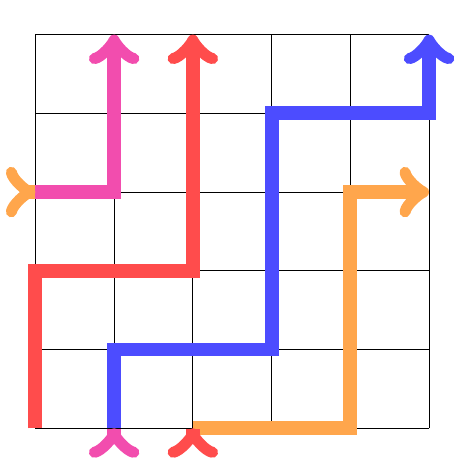
\begin{tikzpicture}
    \draw (0,0) grid (5,5);
    \draw[line width=5, ->, red!70] (0,0)--(0,2)--(2,2)--(2,5);
    \draw[line width=5, ->, orange!70] (2,0)--(4,0)--(4,3)--(5,3);
    \draw[line width=5, ->, red!70] (2,-0.01)--(2,0);
    \draw[line width=5, ->, magenta!70] (0,3)--(1,3)--(1,5);
    \draw[line width=5, ->, orange!70] (-0.01,3)--(0,3);
    \draw[line width=5, ->, blue!70] (1,0)--(1,1)--(3,1)--(3,4)--(5,4)--(5,5);
    \draw[line width=5, ->, magenta!70] (1,-0.01)--(1,0);
  \end{tikzpicture}
  \caption{An example of a walk on a $5 \times 5$ torus that touches every lattice point.}
\end{figure}

\begin{question}
  How many such walks exist?
\end{question}

\begin{related}
  \item What if the walks must touch every lattice point?
  \item What if the walks must wrap around the torus exactly $k$ times?
  (For $k = 1$ and $m = n$, this is the number of walks along the edges of an
  $n \times n$ non-toroidal grid.)
  \item What if there always must be weakly more ``up'' steps than ``right''
    steps? (generalization of staying above the diagonal) Strongly more?
  \item What if this is done on a cylinder? M\"obius strip? More dimensions?
  \item What if walks can intersect at a right angle? What if there must be exactly $k$ intersections?
  \item What if more general loops were counted? (i.e. any walk from $(0,0)$ to $(0,m), (n,0)$ or $(n,m)$.)
\end{related}

\begin{references}
  \item Problem 92.
\end{references}

\end{document}
